\setcounter{step}{0}
%------------------------------------------
% information doc
\subsection{Obrátené rezne}
%------------------------------------------

\begin{ingredient}
%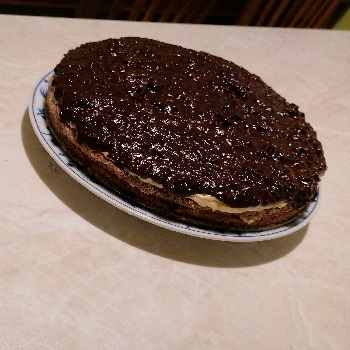
\includegraphics[height=5.5cm]{images/daim}
\def\portions{4}%
\textbf{{\normalsize Ingrediencie (\portions porcie):}}
%\vspace{0.5cm}
\begin{main}
	\item bravčové mäso
	\item olej
	\item soľ
	\item čierne korenie
	\item strúhanka
	\item vajcia
	\item cibuľa
\end{main}
\begin{subingredient}{Nálev}
	\item maslo
	\item olej
	\item soľ
	\item vegeta
	\item kečup
	\item horčica
	\item čierne korenie
\end{subingredient}
\end{ingredient}
\begin{recipe}
\textbf{{\normalsize Príprava:}}
\begin{enumerate}

\item{Mäso naklepeme a nakoreníme}
\item{Do mäsa vkepeme strúhanku}
\item{Namočíme vo vajíčku a sprudka opražíme}	
\item{Vymastiť plech}
\item{Pokrájať cibuľu na kolieska a poukladať na rezne na plech}
\item{Pripravíme nálev:}
\begin{enumerate}
\item{Rozpustiť maslo s olejom}
\item{Pridať soľ, vegetu, kečup, horčicu, korenie}
\item{Prevariť na sporáku}
\end{enumerate}
\item{Vyliať na rezne}
\item{Zakryť alobalom a dať piecť}
\item{5 minút na najsilnejšom}
\item{20-30 minút na 180°C}
\item{5 minút bez alobalu}

\end{enumerate}
\end{recipe}

\begin{notes}

\end{notes}
\clearpage	